%
% Modo de operación ECB, capítulo de antecedentes.
% Proyecto Lovelace.
%

\subsubsection{\acrfull{gl:ecb}}

La figura \ref{figura:ecb} muestra un diagrama esquemático de este modo de
operación. Según la ecuación \ref{modo_de_operacion}, el algoritmo recibe a la
entrada una llave y un mensaje de longitud arbitraria: la llave se pasa
sin ninguna modificación a cada función del cifrado por bloques; el mensaje
se debe de partir en bloques ($ T = B_1 || B_2 || \dots || B_n $).

\begin{figure}[H]
  \centering
  \begin{subfigure}{0.45\textwidth}
      \begin{center}
          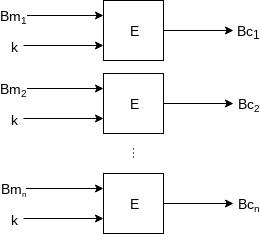
\includegraphics[width=0.7\linewidth]
            {contenidos/antecedentes/bloques/modos/diagramas/modo_ecb.png}
          \caption{Cifrado.}
      \end{center}
  \end{subfigure}
  \begin{subfigure}{0.45\textwidth}
      \begin{center}
          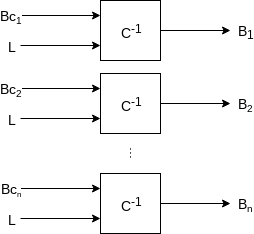
\includegraphics[width=0.7\linewidth]
            {contenidos/antecedentes/bloques/modos/diagramas/modo_ecb_inverso.png}
          \caption{Descifrado.}
      \end{center}
  \end{subfigure}
  \caption{Modo de operación \acrshort{gl:ecb}.}
  \label{figura:ecb}
\end{figure}

\begin{pseudocodigo}[caption={Modo de operación \acrshort{gl:ecb}, cifrado.}]
  entrada: llave $ L $; bloques de mensaje $ B_1, B_2 \dots B_n $.
  salida:  bloques de mensaje cifrado $ Bc_1, Bc_2 \dots Bc_n $.
  inicio
    para_todo $B$
      $Bc_i$ $\gets$ C($L$, $B_i$)
    fin
    regresar $Bc$
  fin
\end{pseudocodigo}

\begin{pseudocodigo}[caption={Modo de operación \acrshort{gl:ecb}, descifrado.}]
  entrada: llave $ L $; bloques de mensaje cifrado $ Bc_1, Bc_2 \dots Bc_n $.
  salida:  bloques de mensaje original $ B_1, B_2 \dots B_n $.
  inicio
    para_todo $Bc$
      $B_i$ $\gets$ $C^{-1}$($L$, $Bc_i$)
    fin
    regresar $B$
  fin
\end{pseudocodigo}
